%begin-include
\section{Software for Ranking of Models of Signaling Networks}
In this section we describe the software we used to perform the ranking
of signaling network models. The first software, SigNetMS, is an 
implementation of the model ranking method presented on 
section~\ref{sec:marginal_likelihood_method}, which estimates the 
marginal likelihood of the data being reproduced by a model.  The second 
software, ABC-SysBio implements the method based on the approximate 
Bayesian Computation, presented on section~\ref{sec:abc_method}.

\subsection{SigNetMS}
To perform the model ranking using an estimate of the marginal 
likelihood, we created the software SigNetMS, which is an acronym of 
{\bf Sig}naling {\bf Net}work {\bf M}odel {\bf S}election. This software
was implemented in Python and it is a free software, under the \emph{GNU 
General Public License}, and available on
\href{https://github.com/gustavoem/SigNetMS}{GitHub}. The SigNetMS 
software can read and parse files containing models of signaling network 
represented in the Systems Biology Markup Language (SBML) format and 
then construct the respective system of differential equations according 
to the chemical species and interactions defined on the file. The 
experiments observations and prior distributions of parameters are 
defined by the user with Extensible Markup Language (XML) files. Four 
other parameters are necessary to run SigNetMS, all of them related to 
the sampling of the power posteriors. 

The method we used to sample each of the power posterior distributions
is the one we presented on section~\ref{sec:power_posteriors_sampling}.
The four parameters related to the sampling determine the size of all
sampling  performed and also the adaptive behaviour of one of the 
Metropolis-Hastings algorithm used. The first parameter defines the 
number of iterations of the first sampling algorithm. This algorithm is 
adaptive because, after a fixed number of iterations, the covariance of 
the jump distribution is updated according to the acceptance rate of 
proposed points; this fixed number of iterations is the second sampling 
parameter. Finally, the third and fourth parameter determine the size of
the second and third sampling steps respectively.

To implement the method we still have to define the proposal 
distributions. Since the proposed model parameters cannot have 
nonpositive values (because they are reaction rate constants), the 
proposal distribution should have a probability density function that 
has value zero for nonpositive numbers. Moreover, its desired, through 
the sampling steps, to control the mean and variance of the proposal 
distributions. For all of the three steps, if the current point of the
chain is $\theta$, then the jump distribution should have mean close
to $\theta$. Also, in the first step, the covariance matrix  of the 
proposal distribution should be proportional to the covariance of 
the prior distribution of parameters. Then, for the two final steps, the 
covariance matrix of the jump distribution should be proportional to an
estimate $\hat{C}$ of the covariance of the parameters, calculated with 
the accepted points of the chain.

In our first attempt, we used multivariate lognormal distributions for 
all the sampling steps. If $X$ is a $MultivariateNormal (\mu, \Sigma)$, 
then $Y = e^{X}$ is $MultivariateLognormal (\mu, \Sigma)$. However, we 
found out that for some combinations of $\theta$ and $\hat{C}$, there 
is no combination of parameters $(\mu, \Sigma)$ such that $Y \propto 
MultivariateLognormal (\mu, \Sigma)$ with $\expectation[Y] = \theta$ and
$var(Y) = \hat{C}$. Then the solution we proposed is to use a truncated 
normal distribution for which only positive numbers have positive 
probability. We can generate a truncated normal random variable, 
$Y \propto TruncatedNormal (\mu, \Sigma)$ by 
repeatedly generating a normal random variable, $X \propto Normal(\mu, 
\Sigma)$ until $X$ is positive. However, this approach has the drawback 
that  $\expectation[Y]$ is usually greater than $\mu$, implying on a 
biased run of Metropolis-Hastings.
{\color{blue} Maybe we should state here that we can't calculate pdf of
the truncated normal distribution?}

The SigNetMS program also has an optional argument that allows the user
to get a verbose run, showing all proposed parameters for each 
temperature as well as the accepted parameters used to estimate the 
logarithm of the marginal likelihood. 

%-> implemented in Python
%-> implements the ABC-SMC method we explained earlier
%-> also reads models in SBML format
\section{ABC-SysBio}
ABC-SysBio is a Python software that implements the Approximate Bayesian
Computation Sequential Monte Carlo (ABC SMC) method~\cite{Liepe2010}. 
This software, similarly to SigNetMS, also takes as input SBML models as 
well as prior distribution of parameters and experimental data. As the 
output, the software returns, for each candidate model, an estimate of 
the probability of that model reproducing the experimental data. The 
source code of the method is available on 
\href{https://sourceforge.net/projects/abc-sysbio/files/}{SourceForge}.

\section{Model Selection Experiments}
The experiments we performed to test both methods consists in taking 
four candidate models and ranking them according to experimental data 
generated by one of them. To generate the simulation data of the 
"correct" model, a set of parameter values, initial concentrations, time 
frames, and a measurement based on the concentration of the chemical 
species are chosen; then, a simulation of the model is generated and the 
artificial measurements are produced, with an introduced Gaussian error 
with mean zero and standard deviation $0.01$. After that, all 
information used to generate data, except initial concentrations, is 
discarded and the models are ranked based on the simulated measurements 
and prior distributions only.

We performed two experiments, the first is presented 
in~\cite{Vyshemirsky2007} and consists of a common structure in signal 
transduction; the second, created for this project, consists of a 
simpler network, containing a few enzymatic reactions and other first 
order chemical interactions.

\subsection{The First Experiment}
\label{sec:experiment_one}
The four candidate models of the first experiment are presented in 
figure~\ref{fig:girolami_models}. The model 1, represented on figure
~\ref{fig:gir_hyp1} is used to generate artificial experimental data
for which all models will be ranked. This network has as components the
degradation of S into dS with reaction rate constant $k_1$; a reversible 
second order reaction \ce{R + S <=> RS} with forward rate constant $k_2$ 
and reverse rate constant of $k_3$; a first order reaction 
\ce{RS -> R_{pp}}; and a Michaelis-Menten (MM) reaction \ce{R_{pp} -> R} 
for which the reaction rate constant and the omitted enzyme 
concentration are combined into one single parameter $V$. Model 2, on 
figure~\ref{fig:gir_hyp2} is a simplification of model 1 in which the
enzymatic reaction of phosphorilation of R is reformulated as a 
MM reaction with enzyme $S$; the other MM reaction, \ce{R_{pp} -> R}, 
now has speed constant $V$ and MM constant $k_3$. Model 3, on figure
\ref{fig:gir_hyp3}, is a simplification of model 2 because it neglects 
the degradation of the chemical species S into dS. The model 4, on 
figure~\ref{fig:gir_hyp4}, is a more complex version of model 1, in 
which the dephosphorylation of R$_{pp}$ is not simplified as a MM 
reaction.

\begin{figure}[H]
  \centering 
  \begin{tabular}{c c}
    \subfigure[]{
    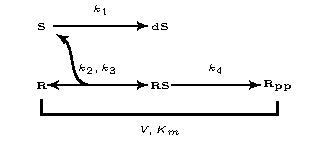
\includegraphics[clip=true,width=.45\linewidth]{experiments/diagrams/bioinformatics_model1.pdf}
    \label{fig:gir_hyp1}}
    &
    \subfigure[]{
    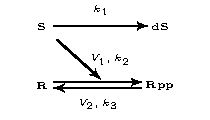
\includegraphics[clip=true,width=.45\linewidth]{experiments/diagrams/bioinformatics_model2.pdf}
    \label{fig:gir_hyp2}} \\
    \subfigure[] {
    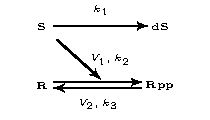
\includegraphics[clip=true,width=.45\linewidth]{experiments/diagrams/bioinformatics_model3.pdf}
    \label{fig:gir_hyp3}}
    &
    \subfigure[] {
    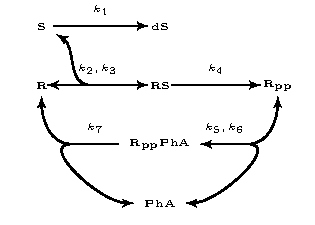
\includegraphics[clip=true,width=.45\linewidth]{experiments/diagrams/bioinformatics_model4.pdf}
    \label{fig:gir_hyp4}}
    \end{tabular}
    \caption{The four models used on the first experiment. The 
    experimental measurement on those models is the concentration of the
    chemical species $R_{pp}$ over time. Model~\ref{fig:gir_hyp1} was
    used to generate artificial experimental data for which those models
    are ranked. Model~\ref{fig:gir_hyp2} is a simplification of the 
    first model in which the phosphorylation of $R$ to $R_{pp}$ was 
    simplified using the Michaelis-Menten kinetics. 
    Model~\ref{fig:gir_hyp4} is a more complex version of the first 
    model. Finally, model~\ref{fig:gir_hyp3} is a very simplified 
    version of the first model, because it neglects the degradation of 
    $S$.}
  \label{fig:girolami_models} 
\end{figure}

The experimental measurement chosen for the hypothesis is the 
concentration of R$_{pp}$ on the time steps: 2s, 5s, 10s, 20s, 40s, 
60s, and 100s. The parameter values chosen for simulation are: 
$k_1 = 0.07$, $k_2 = 0.6$, $k_3 = 0.05$, $k_4 = 0.3$, $V = 0.017$, and
$K_m = 0.3$. The initial concentrations are: S $= 1$, R $= 1$, dS $= 0$,
RS $= 0$, R$_{pp} = 0$. {\color{blue}TODO: Why can I omit the unit of 
concentrations and reaction rate?} The model is then simulated and a 
Gaussian error with mean zero and standard deviation $0.01$ is added to 
the simulation data; this procedure is repeated three times and hence 
produces three experimental observations. 
Figure~\ref{fig:girolami_simulation} shows one of the experimental 
observations.
\begin{figure}
    \begin{center}
    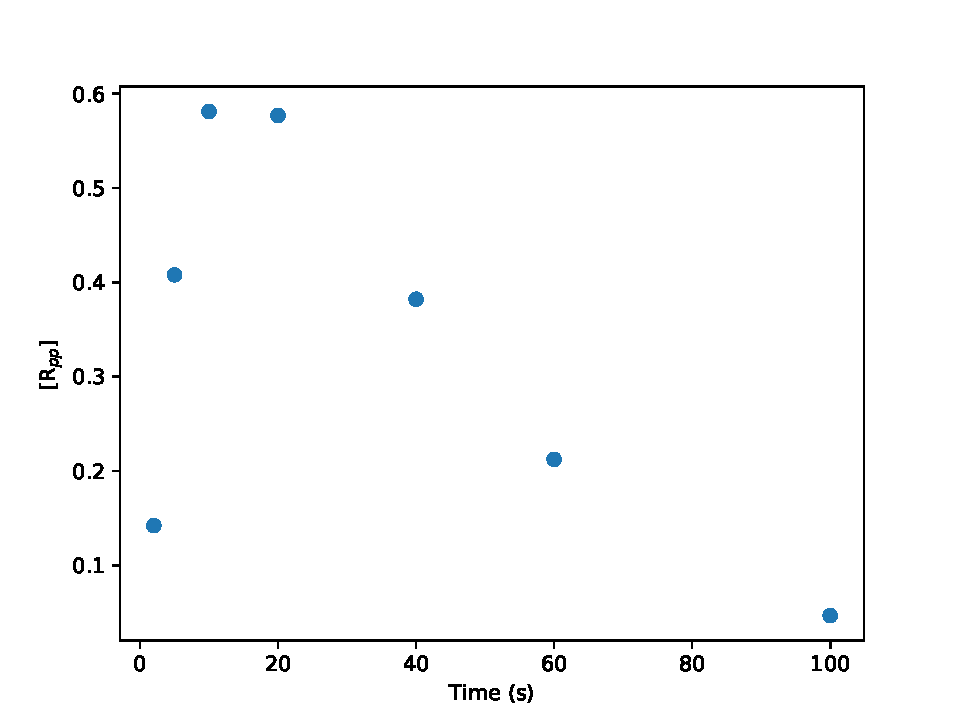
\includegraphics[width=.75\textwidth]{experiments/simulations/girolami_data.pdf}
    \caption{Artificial experimental observation generated with model 1.}
    \label{fig:girolami_simulation}
    \end{center}
\end{figure}

%We chose two sets of prior distributions to use in this experiment.
%The first is using Gamma, while in the second we used Lognormal priors.

\subsection{The Second Experiment}
The second experiment were created for this project and it consists in a
problem with simpler hypothesis than experiment 1. The four candidate
models are presented in figure~\ref{fig:smallest_models}. The model 1
is the one used to generate the artificial experimental data. This model
is presented on figure~\ref{fig:sma_hyp1} and it is composed by a 
reversible reaction \ce{A + B <=> AB} with forward rate constant $k_1$ 
and reverse rate constant $k_2$; an enzymatic reaction \ce{B -> C} with 
Michaelis constant $K_4$ and with omitted enzyme concentration and 
catalytic rate constant combined into a single parameter $V5$; and 
another enzymatic reaction \ce{C -> B} with catalytic action of AB. 
Model 2, presented on figure~\ref{fig:sma_hyp2} is a simplification of
the first model that do not consider the enzymatic reaction that 
transforms B into C. Model 3, presented on figure~\ref{fig:sma_hyp3} is
a generalization of the first model that adds an enzymatic reaction that
can transform C into A, with Michaelis constant $K_{5m}$ and has 
catalytic rate constant combined with the omitted enzyme concentration 
into the parameter $V_5$. Model 4, presented on 
figure~\ref{fig:sma_hyp4}, is a spurious version of model 1, since it 
inverts the two enzymatic reactions between B and C. Model 4 is going to
be used as a control model as it should have the worst ranking between
all models.


\begin{figure}[H]
  \centering 
  \begin{tabular}{c c}
    \subfigure[]{
    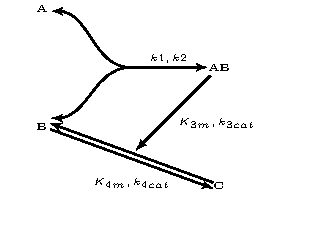
\includegraphics[clip=true,width=.45\linewidth]{experiments/diagrams/smallest_model1.pdf}
    \label{fig:sma_hyp1}}
    &
    \subfigure[]{
    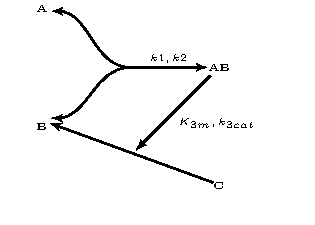
\includegraphics[clip=true,width=.45\linewidth]{experiments/diagrams/smallest_model2.pdf}
    \label{fig:sma_hyp2}} \\
    \subfigure[] {
    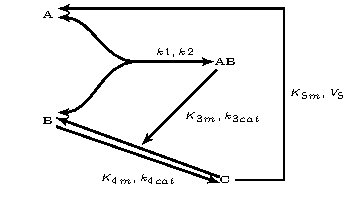
\includegraphics[clip=true,width=.45\linewidth]{experiments/diagrams/smallest_model3.pdf}
    \label{fig:sma_hyp3}}
    &
    \subfigure[] {
    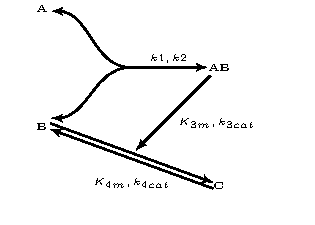
\includegraphics[clip=true,width=.45\linewidth]{experiments/diagrams/smallest_model4.pdf}
    \label{fig:sma_hyp4}}
    \end{tabular}
    \caption{The four models used on the second experiment. The 
    experimental measurement used for these models is the concentration
    of the chemical species B. Model~\ref{fig:sma_hyp1} was
    used to generate artificial experimental data for which these models
    are ranked. Model~\ref{fig:sma_hyp2} is a simplification of the 
    first model, removing the enzymatic reaction that B into C. 
    Model~\ref{fig:sma_hyp3} is a generalization of the first model, and
    it is more complex too. Model~\ref{fig:sma_hyp4} inverts the two
    enzymatic reactions that are happening between B and C, this 
    hypothesis is the control as it should give the worst fit to 
    experimental data.}
  \label{fig:smallest_models} 
\end{figure}

The simulation measurement used on this experiment is to take the 
concentration of the chemical species B over the time steps: 0s, 142s,
285s, 428s, 571s, 714s, 857s, and 1000s. We simulated model 1 with 
parameter values: $k_1 = 1.7e-4$, $k_2 = 0.4$, $k_{cat3} = 2$, 
$K_{3m} = 1.43e3$, $V_4 = 1$ and $K_{4m} = 1.07e2$; the initial 
concentrations used were: $A = 200$, $B = 20$, $AB = 0$, $C = 200$.
Again, similarly to what was done on the first experiment, the model 1
generates an artificial measurement to which a Gaussian error, with 
mean zero and standard deviation $0.01$, is added, yielding three 
observations of the model on the specified time steps. 
Figure~\ref{fig:sma_simulation} shows one of these observations.


\begin{figure}
    \begin{center}
    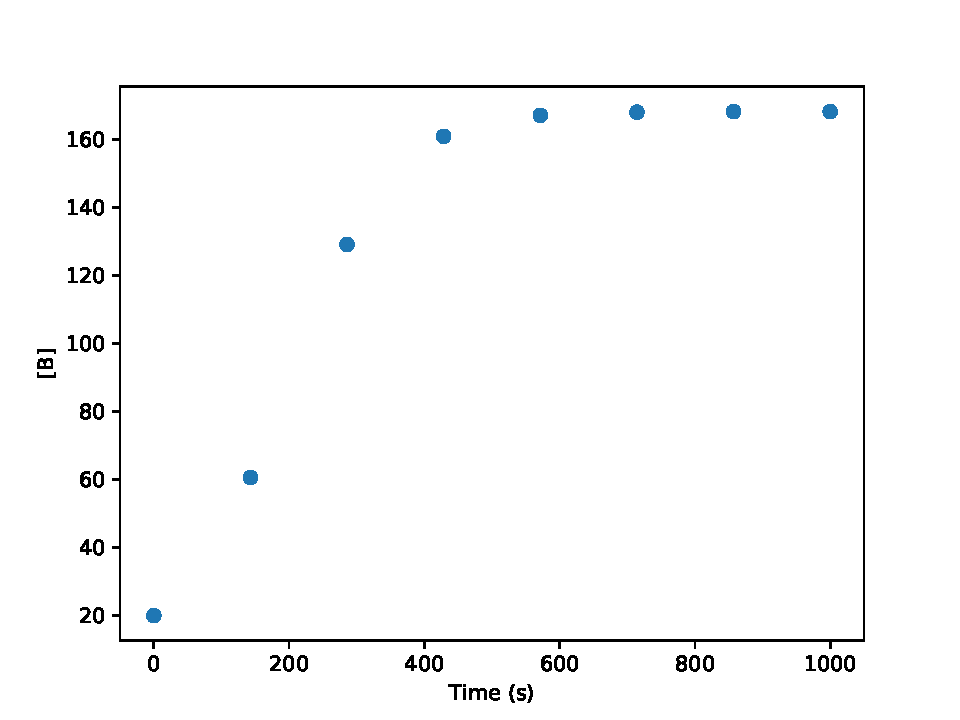
\includegraphics[width=.75\textwidth]{experiments/simulations/smallest_data.pdf}
    \caption{Artificial experimental observation generated with model 1 
        on the second experiment.}
    \label{fig:sma_simulation}
    \end{center}
\end{figure}


\section{Results}

\subsection{Results on the First Experiment}
We performed the first experiment using a setup similar to the work of
Vyshemirsky and Girolami (2007) when they presented the 
Annealing-Melting Integration method~\cite{Vyshemirsky2007}. 
In this experiment, we are expected to achieve the same ranking as 
Vyshemirsky and Girolami, which is 1, 4, 2, 3 from the best to the worst 
model. We already showed part of the set up by showing the candidate 
models, the artificial data generation procedure and initial 
concentrations on section~\ref{sec:experiment_one}. Now we also define 
the prior distributions we used. 

We started the experiment following the work of Vyshemirsky and Girolami
(2007), therefore we defined all model prior parameters as 
$Gamma (1, 3)$. According to the authors, even though the distribution 
has a mean ($\mu = 3$), significantly larger than any of the parameters
used, the results were satisfactory using their methodology. However,
as we will show in the results, using $Lognormal (1, 0.2)$ priors, more 
concentrated on the real parameters, allowed us to achieve better 
results in the software we tested. 


\subsubsection{Results with Gamma priors using ABC-SysBio}
We used the ABC-SysBio software using the automatic iteration scheduler,
which created 26 populations of parameter values, each of them with 100
individual parameters values. At the last iteration, the algorithm 
stopped with $\epsilon = 1$ and the following estimates: 
$\hat{p} (M = 1 | D) = 0.005$, $\hat{p} (M = 2 | D) = 0.014$, 
$\hat{p} (M = 3 | D) = 0.976$ and $\hat{p} (M = 4 | D) = 0.003$. These
estimates induces the ranking 3, 2, 1, 4, which is almost the inverted
ranking obtained by Vyshemirsky and Girolami: 1, 4, 2, 3. 

To understand why this happened, we produced a few graphs that show how
the population of parameters evolve as the number of iterations 
increase. The 
figures~\ref{fig:abc_bio_avgsim1}~and~\ref{fig:abc_bio_avgsim3} show the 
evolution of the simulations generated by the population of parameters 
of different iterations, comparing models 1 and 3, which are 
respectively the true model and the model ranked best by this experiment 
on ABC-SysBio. We can see on these figures that parameters of further 
iterations do imply in better simulation for model 1, while for model 3 
parameters tend to generate a simulation for which the concentration of
R$_{pp}$ stays constant and ``in the middle'' of the experimental 
values. To understand why this happens, we also plotted the actual 
simulations that generated these mean values.

\begin{figure}[h]
  \centering 
  \begin{tabular}{c c}
    \subfigure[]{
    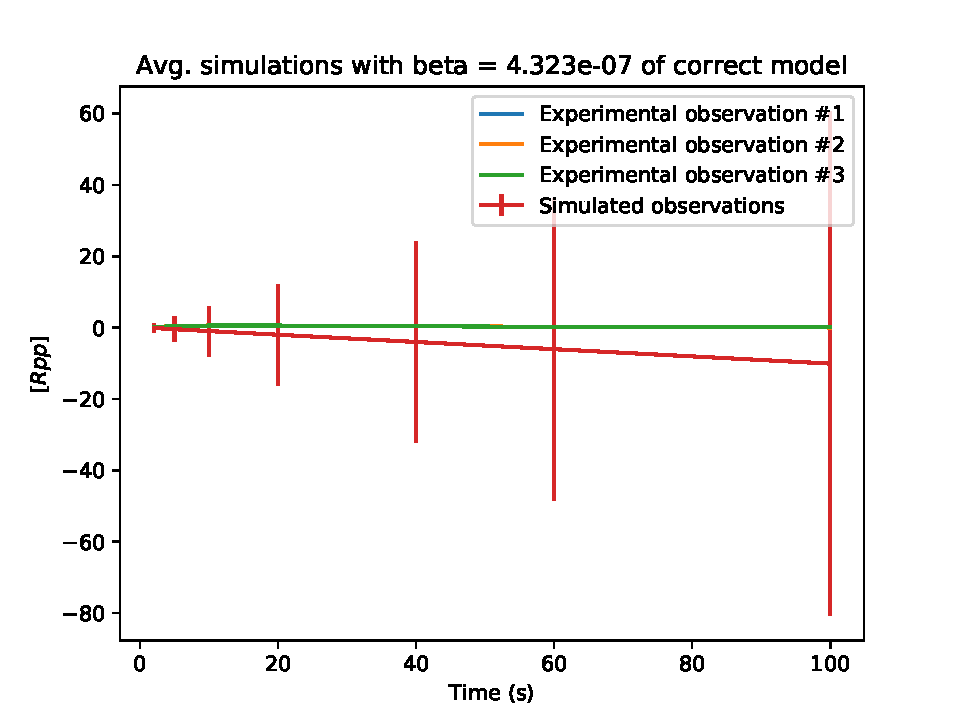
\includegraphics[clip=true,width=.45\linewidth]{experiments/results/girolami/gamma/simulations_model1_1.pdf}
    \label{fig:abc_bio_avgsim1_it1}}
    &
    \subfigure[]{
    \includegraphics[clip=true,width=.45\linewidth]{experiments/results/girolami/gamma/simulations_model1_10.pdf}
    \label{fig:abc_bio_avgsim1_it2}} 
    \\
    \subfigure[]{
    \includegraphics[clip=true,width=.45\linewidth]{experiments/results/girolami/gamma/simulations_model1_20.pdf}
    \label{fig:abc_bio_avgsim1_it3}} 
    &
    \subfigure[]{
    \includegraphics[clip=true,width=.45\linewidth]{experiments/results/girolami/gamma/simulations_model1_26.pdf}
    \label{fig:abc_bio_avgsim1_it4}} 
    \end{tabular}
    \caption{Average simulation generated by model 1 on each iteration
    indicated. For each iteration, the average simulation is created by 
    taking all individuals that are associated to model 1 and evaluating
    the model with these parameters.}
  \label{fig:abc_bio_avgsim1} 
\end{figure}

\begin{figure}[p]
    \centering
    \begin{tabular}{c c}
    \subfigure[]{
    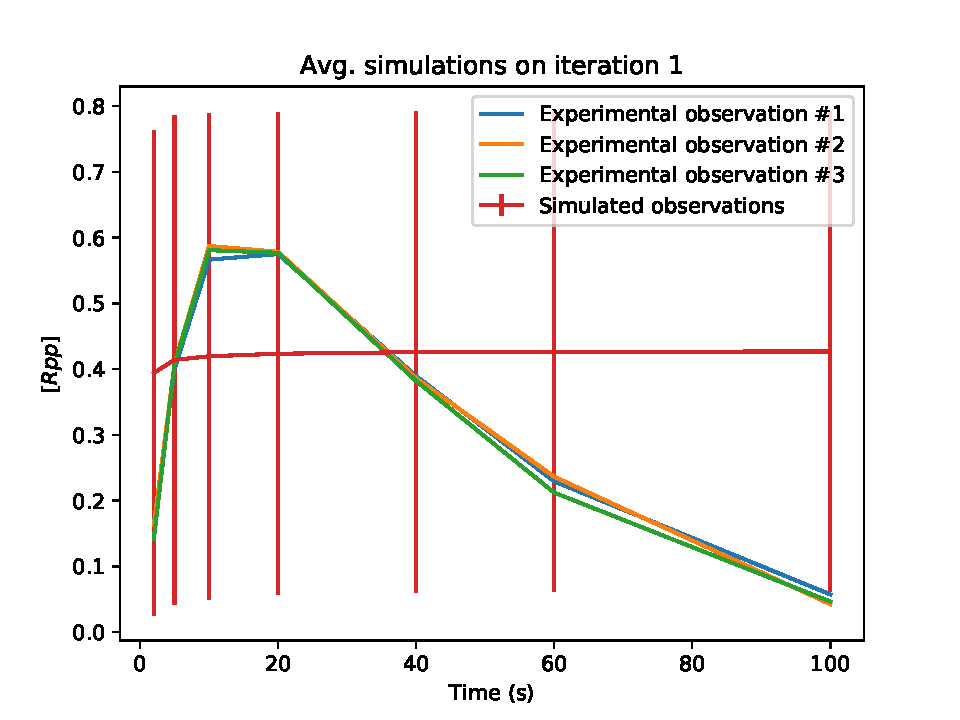
\includegraphics[clip=true,width=.45\linewidth]{experiments/results/girolami/gamma/simulations_model3_1.pdf}
    \label{fig:abc_bio_avgsim3_it1}}
    &
    \subfigure[]{
    \includegraphics[clip=true,width=.45\linewidth]{experiments/results/girolami/gamma/simulations_model3_10.pdf}
    \label{fig:abc_bio_avgsim3_it2}} 
    \\
    \subfigure[]{
    \includegraphics[clip=true,width=.45\linewidth]{experiments/results/girolami/gamma/simulations_model3_20.pdf}
    \label{fig:abc_bio_avgsim3_it3}} 
    &
    \subfigure[]{
    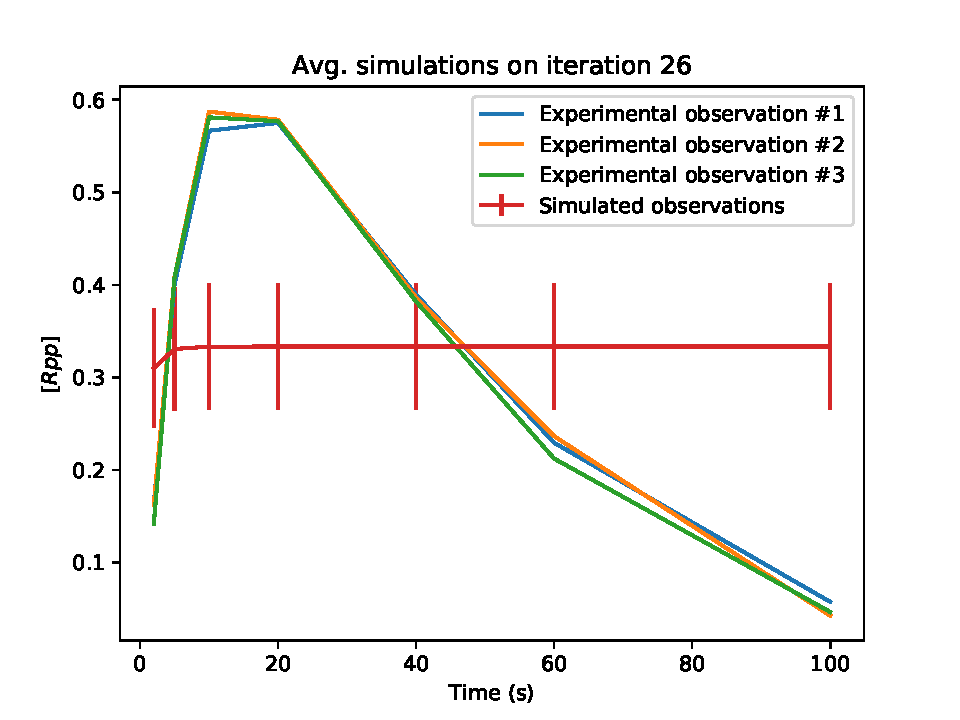
\includegraphics[clip=true,width=.45\linewidth]{experiments/results/girolami/gamma/simulations_model3_26.pdf}
    \label{fig:abc_bio_avgsim3_it4}} 
    \end{tabular}
    \caption{Continuation of figure~\ref{fig:abc_bio_avgsim1}, but 
    average simulations are from model 3. Note that there is a 
    concentration of the simulations around an intermediary value 
    between a high and low concentration of R$_{pp}$.}
    \label{fig:abc_bio_avgsim3}
\end{figure}

On figure~\ref{fig:abc_bio_allsim} we can see the simulation of all 
individuals of model 1 and 3 of the populations of iteration 20 and 26.
Through the red translucent lines of the graph we are able to see 
simulations generated by all parameters of a model in a specific 
iteration. We can observe that there is a clear concentration of 
simulations with a mean concentration value for model 3, while for model
1 there is just a trend that simulations generate curves that are close
to experimental values. More than that, an important information that we
should take from this graph is that the number of lines on the graph
of a model represent the number of individuals of that model in a 
certain iteration. With that, we can note that the majority of 
individuals of the iterations showed on the graphs are from model 3, 
which explains why this model has greater ranking than model 1.

To understand why there are less parameters of model 1 than there are
of model 3 in the last iterations we must recall the dynamics of the
ABC-SMC algorithm. To constroy the population of the next iteration, the
algorithm takes only the parameters from the current population that 
were accepted, i.e. parameters that imply in simulations that dist at 
most some $\epsilon$ from the model. Because of that, if a model has few
individuals accepted in the current population, then there is a high 
chance that there will be few individuals of this model in the next 
population. Therefore, if model 1 had a ``bad start'', with few 
parameters accepted in the early iterations, while model 3 had a ``good
start'', caused by the big $\epsilon$ of first iterations, then this can
be the reason why model 3 has been ranked first.

The ``bad start'' of model 1 may have been caused by the prior 
distribution used, which is not very concentrated around good parameter
values, causing the first model to have many bad performing parameters
in the first populations. Because of that, we decided to do this 
experiment again on ABC-SysBio, but using priors $Lognormal (1, 0.2)$.

\begin{figure}[H]
    \centering
    \begin{tabular}{c c}
    \subfigure[]{
    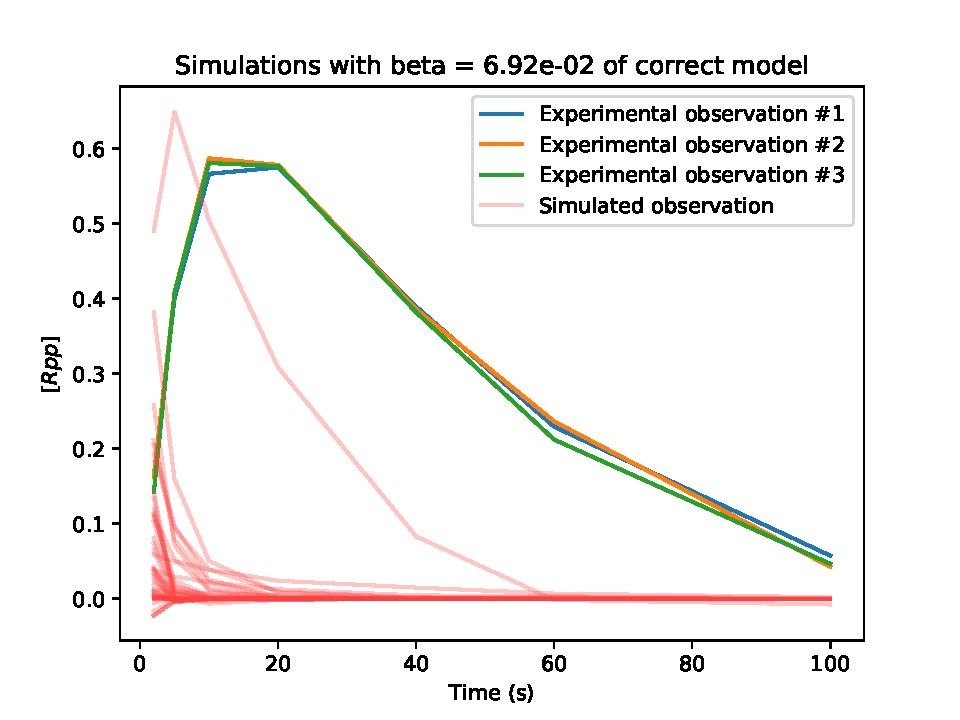
\includegraphics[clip=true,width=.45\linewidth]{experiments/results/girolami/gamma/msimulations_model1_20.pdf}
    \label{fig:abc_bio_allsim1_it20}}
    &
    \subfigure[]{
    \includegraphics[clip=true,width=.45\linewidth]{experiments/results/girolami/gamma/msimulations_model1_26.pdf}
    \label{fig:abc_bio_allsim1_it26}} 
    \\
    \subfigure[]{
    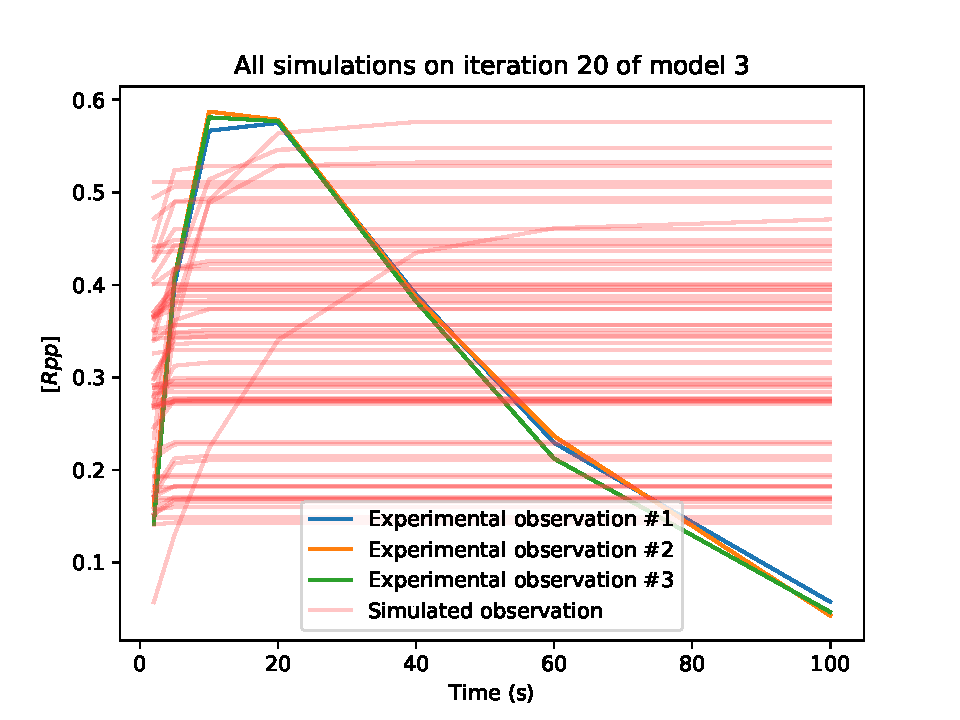
\includegraphics[clip=true,width=.45\linewidth]{experiments/results/girolami/gamma/msimulations_model3_20.pdf}
    \label{fig:abc_bio_allsim3_it20}} 
    &
    \subfigure[]{
    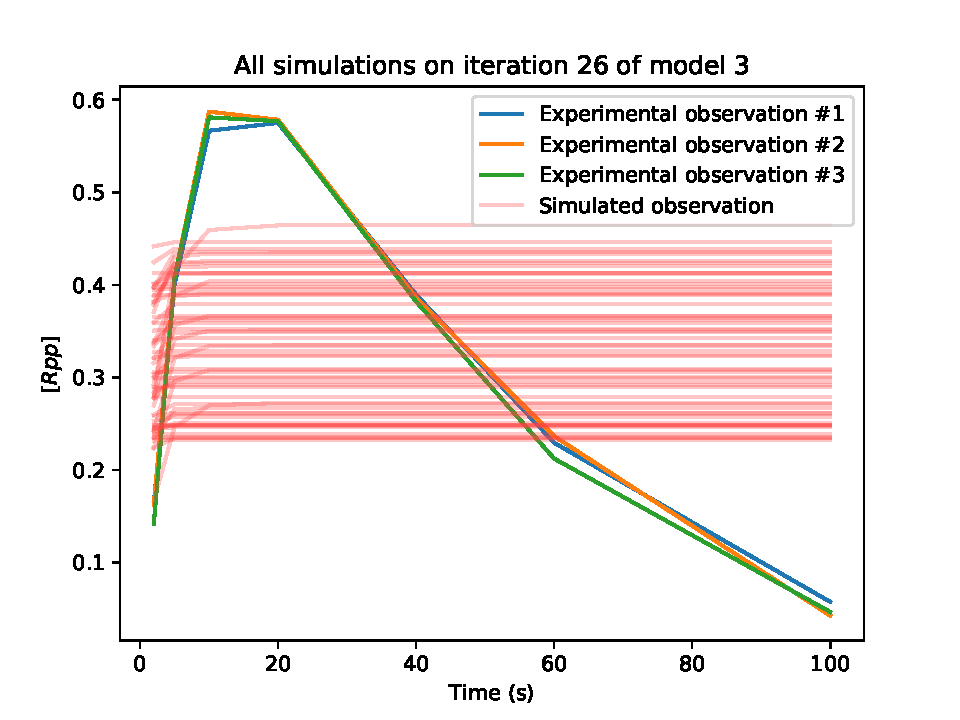
\includegraphics[clip=true,width=.45\linewidth]{experiments/results/girolami/gamma/msimulations_model3_26.pdf}
    \label{fig:abc_bio_allsim3_it26}} 
    \end{tabular}
    \caption{Simulations generated by parameters of iteration 20 and 
    iteration 26 of the ABC-SysBio run. Red translucid lines show the 
    simulation of a single parameter. Stronger red color means 
    overlapping points between simulations.
    Figures~\ref{fig:abc_bio_allsim1_it20}~and~\ref{fig:abc_bio_allsim3_it26}
    show individuals of model 1 while 
    figures~\ref{fig:abc_bio_allsim3_it20}~and~\ref{fig:abc_bio_allsim3_it26}
    show individuals of model 3.
    }
    \label{fig:abc_bio_allsim}
\end{figure}

%\subsubsection{Results with Gamma priors using SigNetMS}
%Using the Gamma prior we also performed the experiment on the SigNetMS
%software. We used this software to estimate the logarithm of the 
%marginal likelihood of each candidate model. The sampling algorithm 
%parameters we used were: 15000 iterations for the first sampling step,
%with covariance updates each 1000 iterations; 5000 iterations for the
%second sampling step; and 5000 iterations on the Populational MCMC step.
%This experiment yielded the following estimates of marginal likelihood:
%$\hat{p} () $

\subsubsection{Results with Lognormal priors using ABC-SysBio}
With the goal of investigating the behaviour of ABC-SysBio when using a 
prior more concentrated on real parameter values, we decided to run the
experiment again using parameter priors distributed as 
$Lognormal (1, 0.2)$. We again ran ABC-SysBio using the automatic 
scheduler with population of size 100. The algorithm stopped after 32
iterations, with final epsilon $\epsilon = 1$, however on iteration 23
the only model present on the populations were from model 1. The 
resulting ranking for this experiment was 1, 4, 3, 2; very similar to 
the ranking presented by Vyshemirsky and Girolami (2007): 1, 4, 2, 3.

The last algorithm iteration that had individuals from all models was 
the 10\textsuperscript{th} iteration. Figure~\ref{fig:abc_bio_log_10it} 
shows the average simulations of all models considering the parameter 
population of iteration 10. We can see that models 1 and 4 perform 
better than models 2 and 3. On the 11\textsuperscript{th} population, no 
parameter of the produced population will be from model 2, and after the 
12\textsuperscript{th} population, no parameter will be from models 3
either. Then, from iteration 12 to 23, only parameters of models 1 and 4
will be on the populations. Model 1 is considered the best fit, as it 
should be by the design of the experiment. 
\begin{figure}[H]
    \centering
    \begin{tabular}{c c}
    \subfigure[]{
    \includegraphics[clip=true,width=.45\linewidth]{experiments/results/girolami/log/simulations_model1_10.pdf}
    \label{fig:abc_bio_log_10it1}}
    &
    \subfigure[]{
    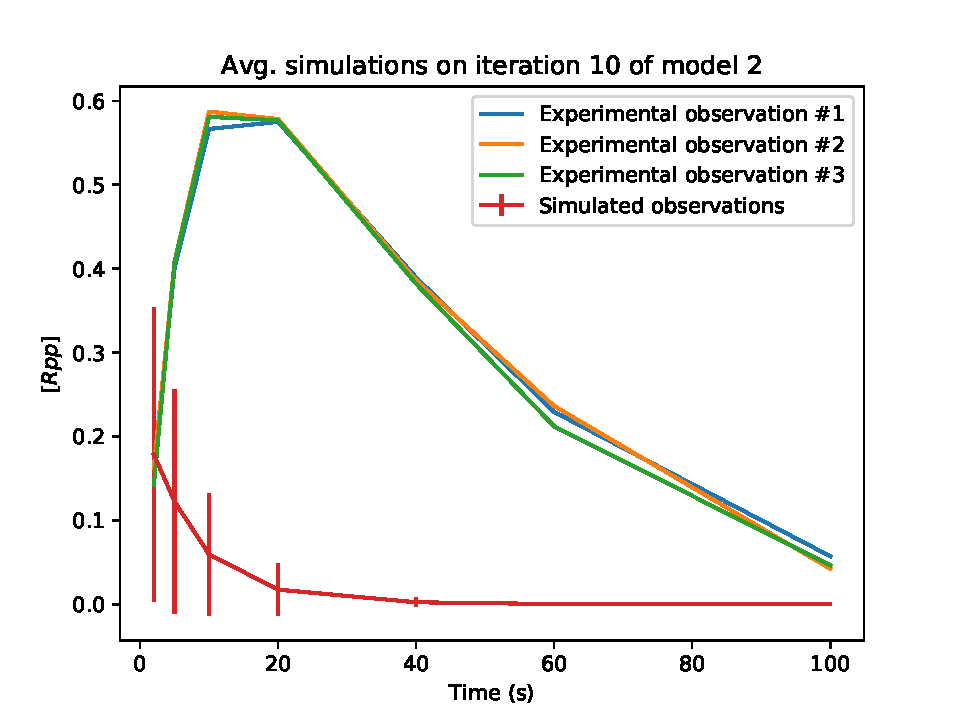
\includegraphics[clip=true,width=.45\linewidth]{experiments/results/girolami/log/simulations_model2_10.pdf}
    \label{fig:abc_bio_log_10it2}} 
    \\
    \subfigure[]{
    \includegraphics[clip=true,width=.45\linewidth]{experiments/results/girolami/log/simulations_model3_10.pdf}
    \label{fig:abc_bio_log_10it3}} 
    &
    \subfigure[]{
    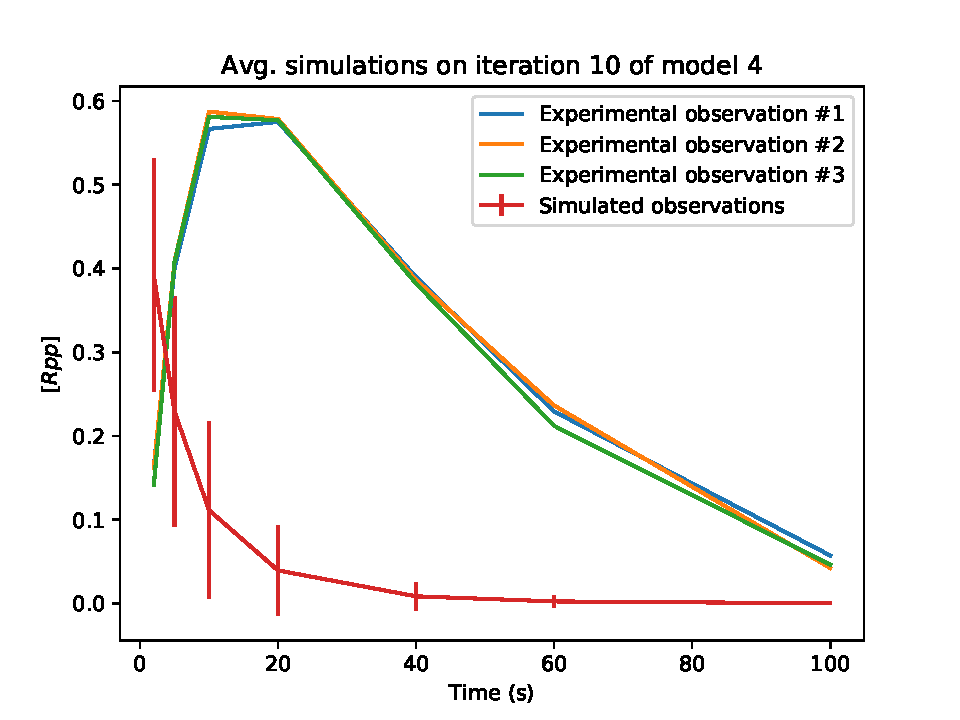
\includegraphics[clip=true,width=.45\linewidth]{experiments/results/girolami/log/simulations_model4_10.pdf}
    \label{fig:abc_bio_log_10it4}} 
    \end{tabular}
    \caption{Average simulation of iteration 10 for all candidate 
    models.}
    \label{fig:abc_bio_log_10it}
\end{figure}

Even tough the ranking produced by the algorithm is reasonably close to
the one produced by Vyshemirsky and Girolami, we decided to plot
new graphs to investigate if the parameters of the populations for model
1 actually bring the simulated results close to the experiments. On 
figure~\ref{fig:abc_bio_log_sims1it26} we present the average and 
individual simulations of model 1 produced by the parameters of this 
model on iteration 26. We can see through the average simulation that 
the mean value for each time step is not close to the experimental 
value, and more than that, we can note on the individual simulations 
plot that the dynamics induced by the parameters are not similar to the 
experimental dynamics. While in the experiments there is a increase and 
then decrease of concentration of R$_{pp}$, in the dynamics induced by 
the found parameters the trend is to have only decrease of 
concentrations of R$_{pp}$ over time. We also plotted an estimation of
the posterior distribution of parameters of model one, presented on 
figure~\ref{fig:posterior_estimate_model1}. This estimative was created
with parameters of model 1 on iteration 26 of the algorithm, and it is
possible to see that the estimated posterior is not concentrated around
the expected values, which should be the parameters values used to 
create the experimental data.

\begin{figure}[H]
    \centering
    \begin{tabular}{c c}
    \subfigure[]{
    \includegraphics[clip=true,width=.45\linewidth]{experiments/results/girolami/log/simulations_model1_26.pdf}
    \label{fig:abc_bio_log_simm1it26}}
    &
    \subfigure[]{
    \includegraphics[clip=true,width=.45\linewidth]{experiments/results/girolami/log/msimulations_model1_26.pdf}
    \label{fig:abc_bio_log_msimm1it26}}
    \end{tabular}
    \caption{Average simulation and individual simulation generated by
    the parameters of model 1 on the 26\textsuperscript{th} iteration.}
    \label{fig:abc_bio_log_sims1it26}
\end{figure}



\begin{figure}[p]
    \centering
    \begin{tabular}{c c}
    \subfigure{
    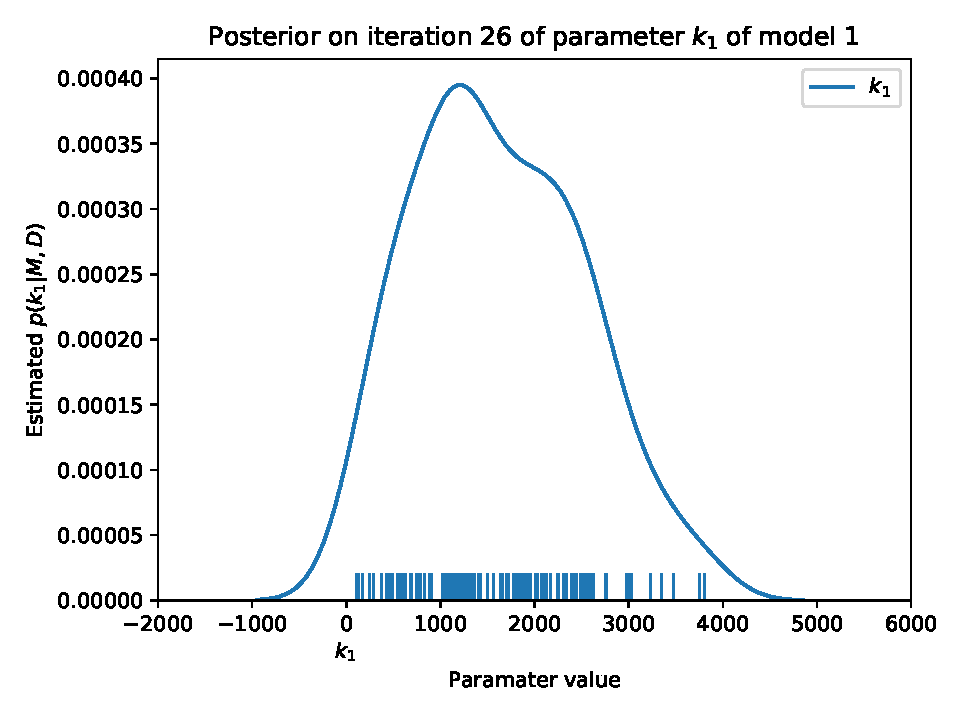
\includegraphics[clip=true,width=.45\linewidth]{experiments/results/girolami/log/model1_26_p0_k_1.pdf}
    %\label{fig:abc_bio_posterior_paramk1}
    }
    &
    \subfigure{
    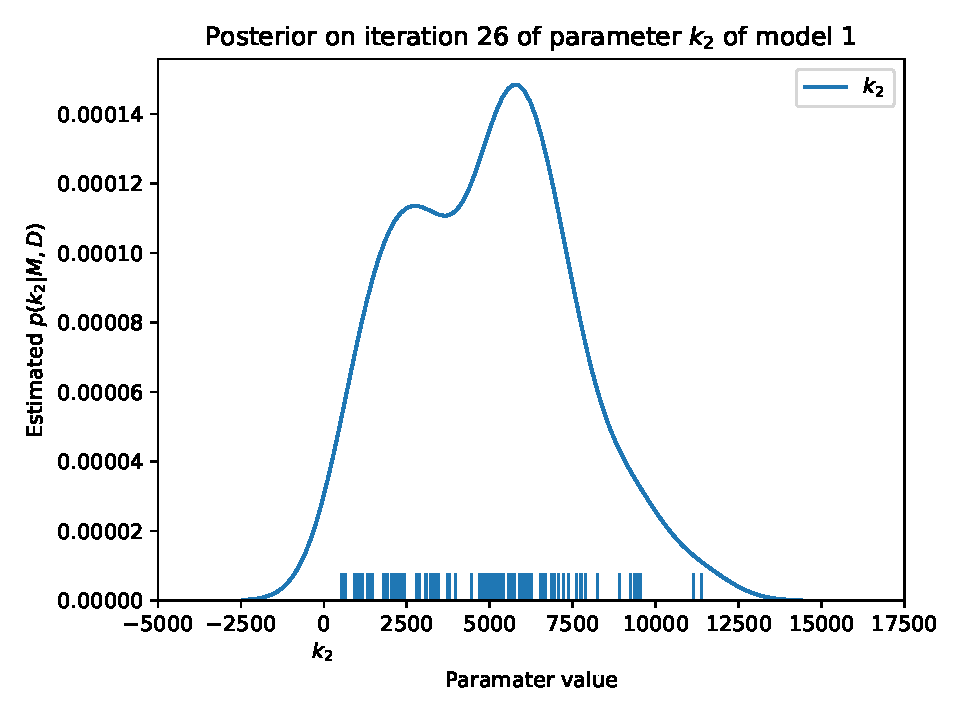
\includegraphics[clip=true,width=.45\linewidth]{experiments/results/girolami/log/model1_26_p1_k_2.pdf}
    %\label{fig:abc_bio_posterior_paramk2}
    }
    \\
    \subfigure{
    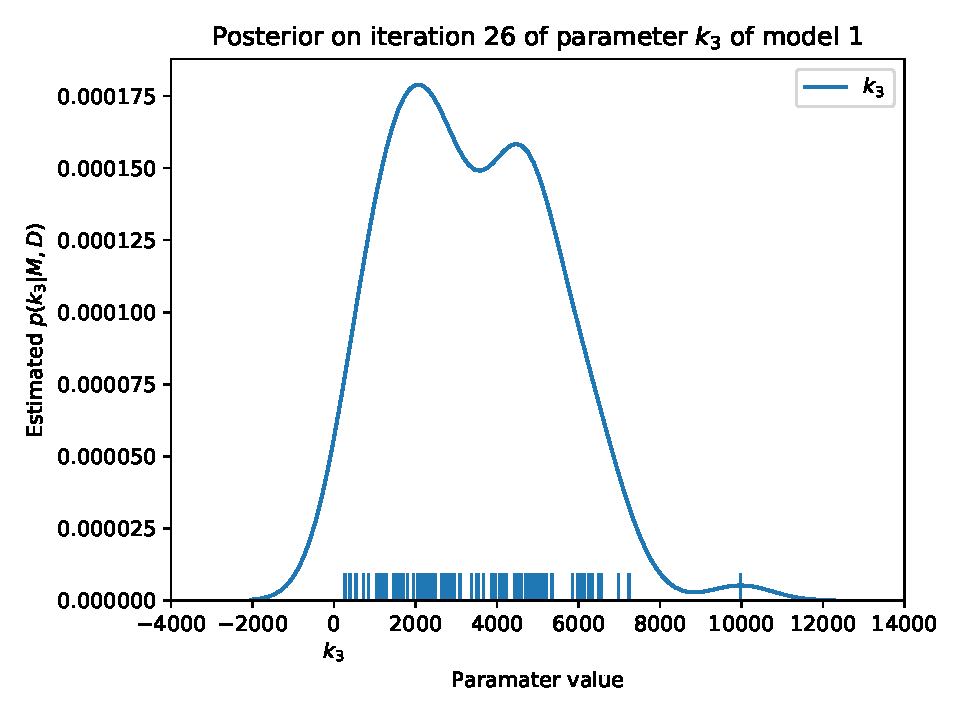
\includegraphics[clip=true,width=.45\linewidth]{experiments/results/girolami/log/model1_26_p2_k_3.pdf}
    %\label{fig:abc_bio_posterior_paramk3}
    }
    &
    \subfigure{
    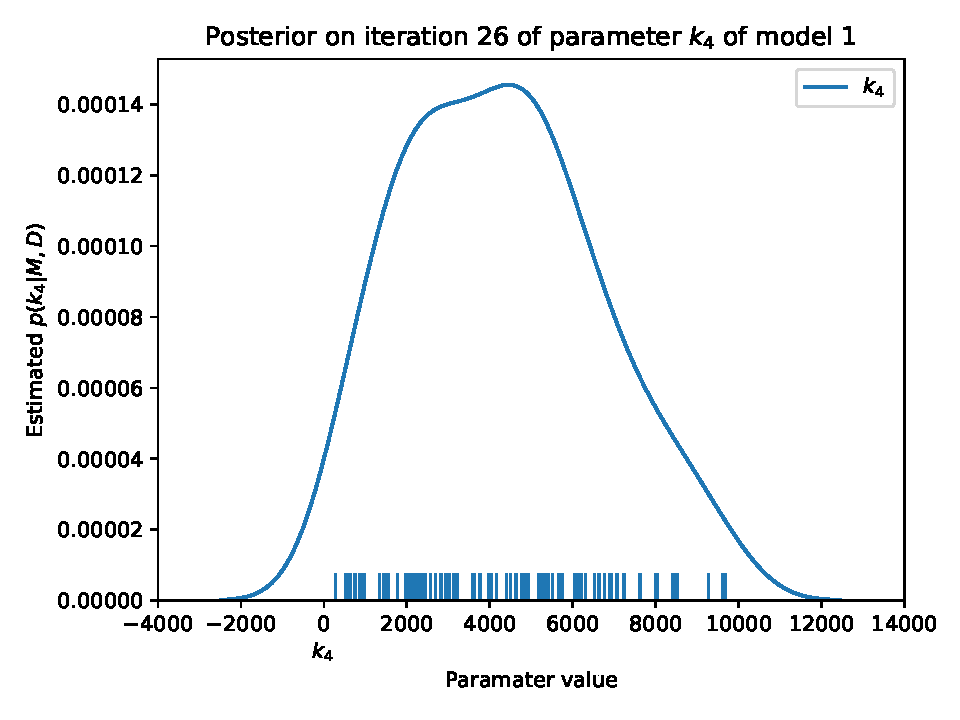
\includegraphics[clip=true,width=.45\linewidth]{experiments/results/girolami/log/model1_26_p3_k_4.pdf}
    %\label{fig:abc_bio_posterior_paramk4}
    }
    \\
    \subfigure{
    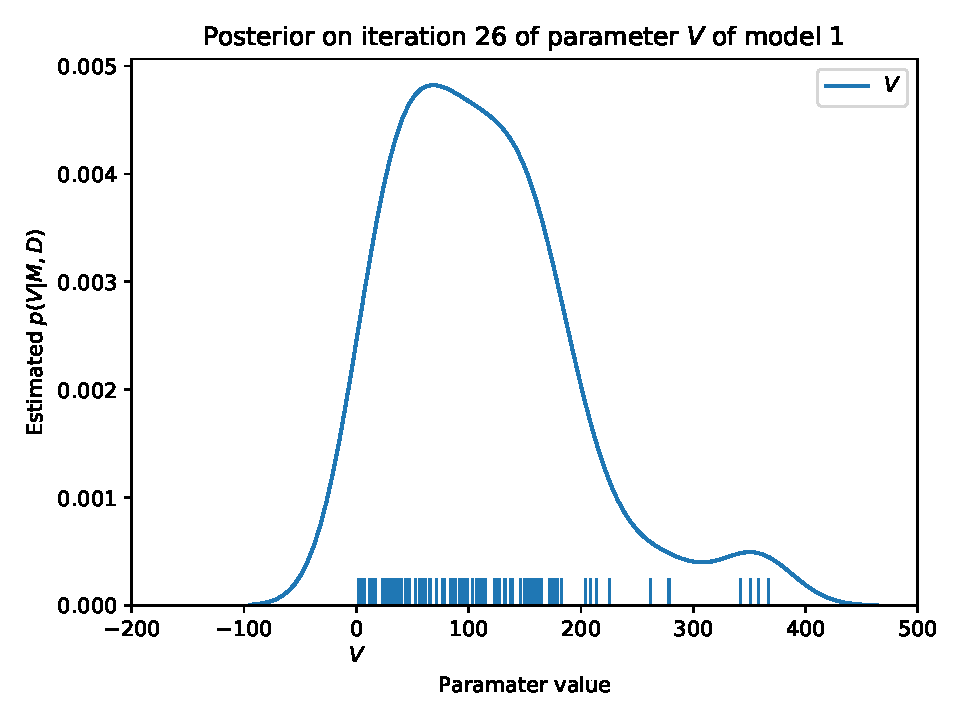
\includegraphics[clip=true,width=.45\linewidth]{experiments/results/girolami/log/model1_26_p4_V.pdf}
    %\label{fig:abc_bio_posterior_paramV}
    }
    &
    \subfigure{
    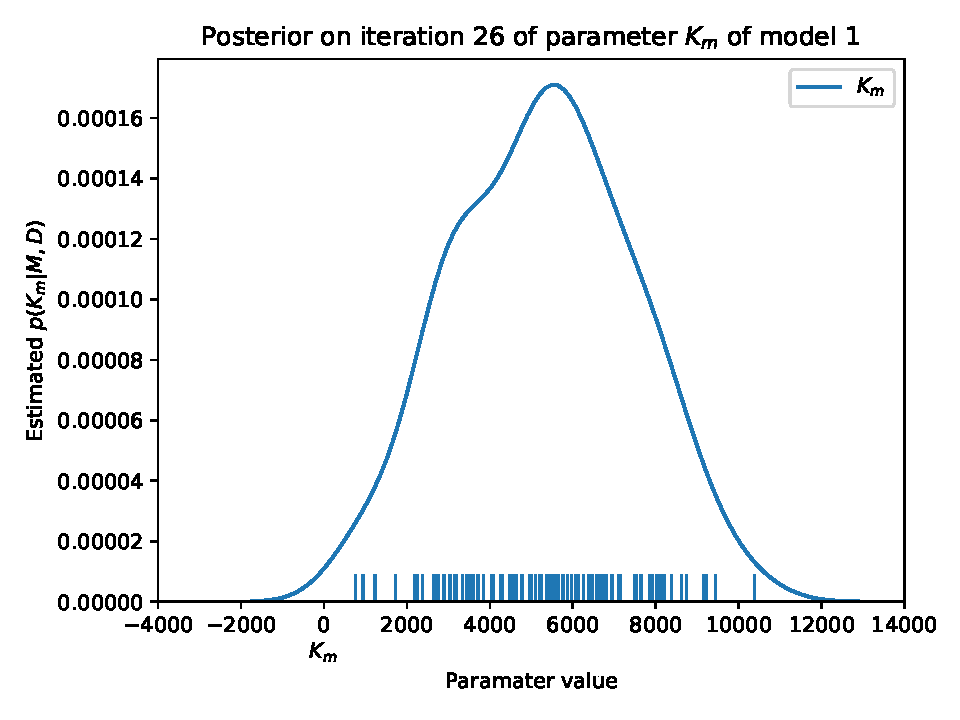
\includegraphics[clip=true,width=.45\linewidth]{experiments/results/girolami/log/model1_26_p5_K_m.pdf}
    %\label{fig:abc_bio_posterior_paramKm}  
    }
    \\
    \end{tabular}
    \caption{Estimates of the posterior distribution of model 1 
    parameters. These estimates were created using the kernel density 
    estimation method from the seaborn Python package. The parameter 
    name on the abscissa of the graph indicates the location of the 
    correct value of the parameter, i.e. the value used to create the 
    experimental data. The estimated posterior is not concentrated
    around the correct parameter values, which are $k_1 = 0.07$, 
    $k_2 = 0.6$, $k_3 = 0.05$, $k_4 = 0.3$, $V = 0.017$.}
    \label{fig:posterior_estimate_model1}
\end{figure}


\subsection{Results on the Second Experiment}
For the second experiment we used only Gamma priors for the model 
parameters. A complete definition of the priors is presented on 
table~\ref{tab:smallest_priors}. We used the ABC-SysBio software to 
perform the model ranking using the automatic $\epsilon$ scheduler with 
a population size of 100 individuals per iteration. As a result, the
ranking produced by the software was: 2, 1, 4, 3. 

\begin{table}[h]
\centering
\begin{tabular}{l l l}
Parameter   & Models     & Prior             \\ \hline
\hline
$k1$        & 1, 2, 3, 4 & $Gamma (1, 0.01)$ \\
$k2$        & 1, 2, 3, 4 & $Gamma (2, 0.5)$  \\
$k_{3cat}$  & 1, 2, 3, 4 & $Gamma (4, 1)$    \\
$K_{3m}$    & 1, 2, 3, 4 & $Gamma (2, 1500)$ \\
$V_4$       & 1, 3, 4    & $Gamma (2, 1)$    \\
$K_{4m}$    & 1, 3, 4    & $Gamma (2, 100)$  \\
$V_5$       & 3          & $Gamma (2, 0.4)$  \\
$K_{5m}$    & 3          & $Gamma (2, 100)$  \\ \hline
\end{tabular}
\caption{Prior distribution for each parameter of models of the second 
    experiment.}
\label{tab:smallest_priors}
\end{table}

The algorithm created 64 iterations until it reached the last iteration
with $\epsilon = 31.03$. After iteration 26, no individuals from the 
populations were from model 3, considered the worst model. After 
iteration 56, no individuals from model 4 were in the populations. Then,
from iterations 56 to 64 only individuals from model 1 and 2 were in 
the populations. In the last population, the estimated probabilities
created by the software were: 
$\hat{p} (M = 1 | D, \epsilon = 31.03) = 0.44$ and 
$\hat{p} (M = 2 | D, \epsilon = 31.03) = 0.56$. Therefore, the result
is inconclusive for which model performs better, 1 or 2. 

On figure~\ref{fig:smallest_all_sim_it20} we show the average of the 
simulations produced by parameters of iteration 20. It is possible to
see that model 3 is indeed performs worse comparing to all other models,
and more than that, the curve produced by model 3 is different from the 
experimental data and curves produces by other models; while in model 3
the concentration of B increases and then decreases, for the other 
models the concentration increases until it stabilizes. On 
figure~\ref{fig:smallest_all_sim_it50} we show the average simulation
of parameters of the 50\textsuperscript{th} iteration of the algorithm.
We can see that models 1 and 2 approximates the curve reasonably well
while model 4, in the other hand, has more error, specially in the 
time steps of 200 and 400 seconds. Finally, on 
figure~\ref{fig:smallest_all_sim_it64} we show the average simulations 
of models 1 and 2 on the 64\textsuperscript{th} iteration of the 
algorithm. We can see that parameters of the last population bring both
models simulations very close to the experimental data.

\begin{figure}[H]
    \centering
    \begin{tabular}{c c}
    \subfigure{
    \includegraphics[clip=true,width=.45\linewidth]{experiments/results/smallest/simulations_model1_20.pdf}
    \label{fig:abc_sma_1it20}}
    &
    \subfigure{
    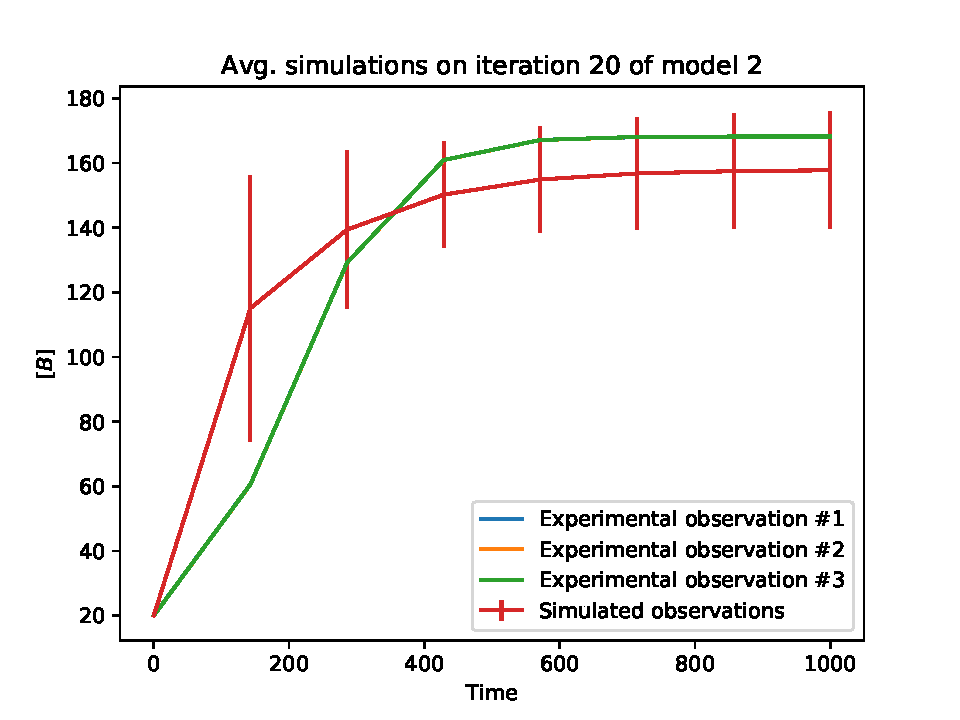
\includegraphics[clip=true,width=.45\linewidth]{experiments/results/smallest/simulations_model2_20.pdf}
    \label{fig:abc_sma_2it20}} 
    \\
    \subfigure{
    \includegraphics[clip=true,width=.45\linewidth]{experiments/results/smallest/simulations_model3_20.pdf}
    \label{fig:abc_sma_3it20}} 
    &
    \subfigure{
    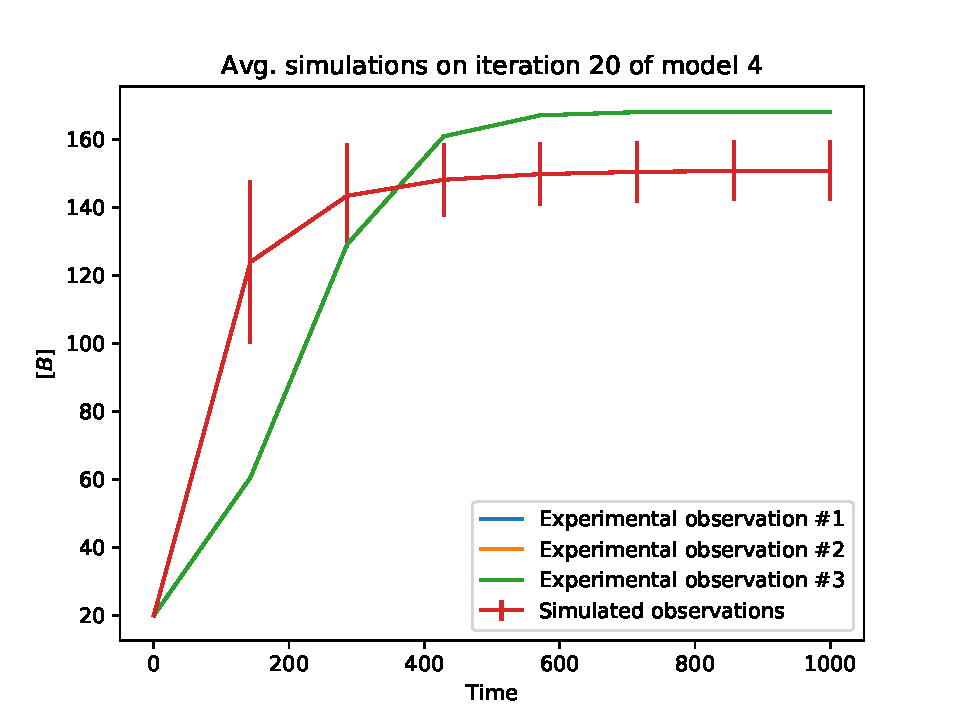
\includegraphics[clip=true,width=.45\linewidth]{experiments/results/smallest/simulations_model4_20.pdf}
    \label{fig:abc_sma_4it20}} 
    \end{tabular}
    \caption{Average simulation of iteration 20 for all candidate 
    models.}
    \label{fig:smallest_all_sim_it20}
\end{figure}

\begin{figure}[p]
    \centering
    \begin{tabular}{c}
    \subfigure{
    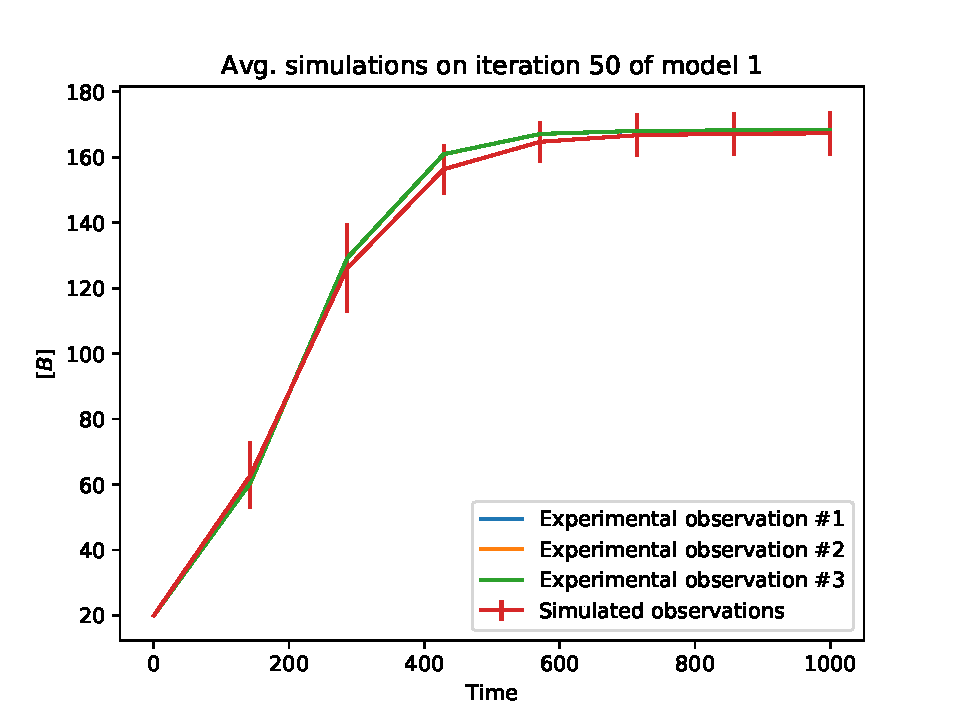
\includegraphics[clip=true,width=.6\linewidth]{experiments/results/smallest/simulations_model1_50.pdf}
    \label{fig:abc_sma_1it50}}
    \\
    \subfigure{
    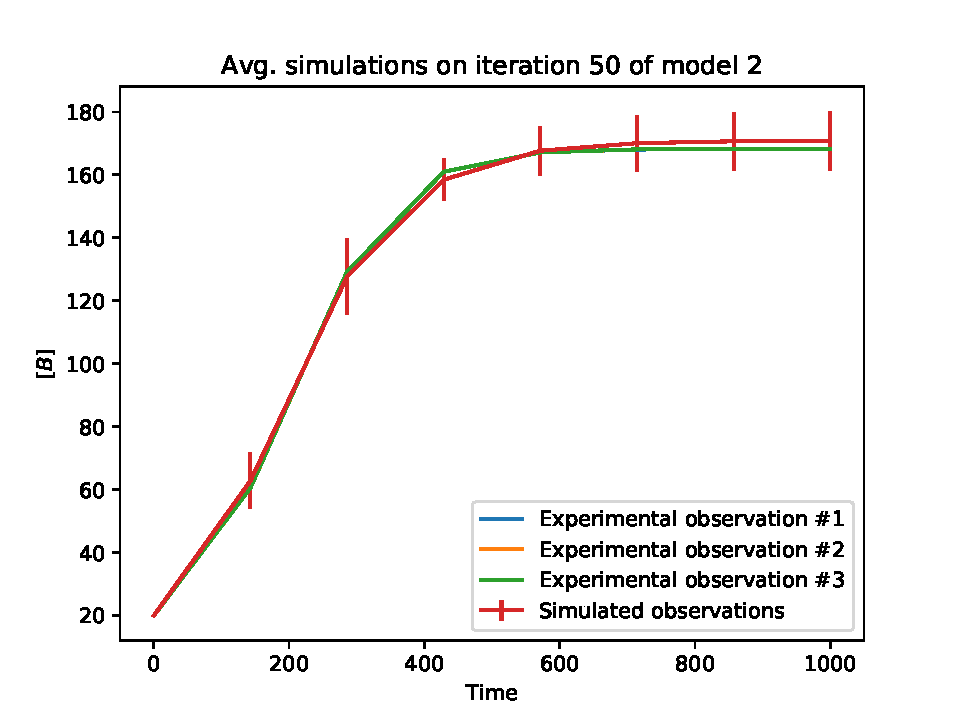
\includegraphics[clip=true,width=.6\linewidth]{experiments/results/smallest/simulations_model2_50.pdf}
    \label{fig:abc_sma_2it50}} 
    \\
    \subfigure{
    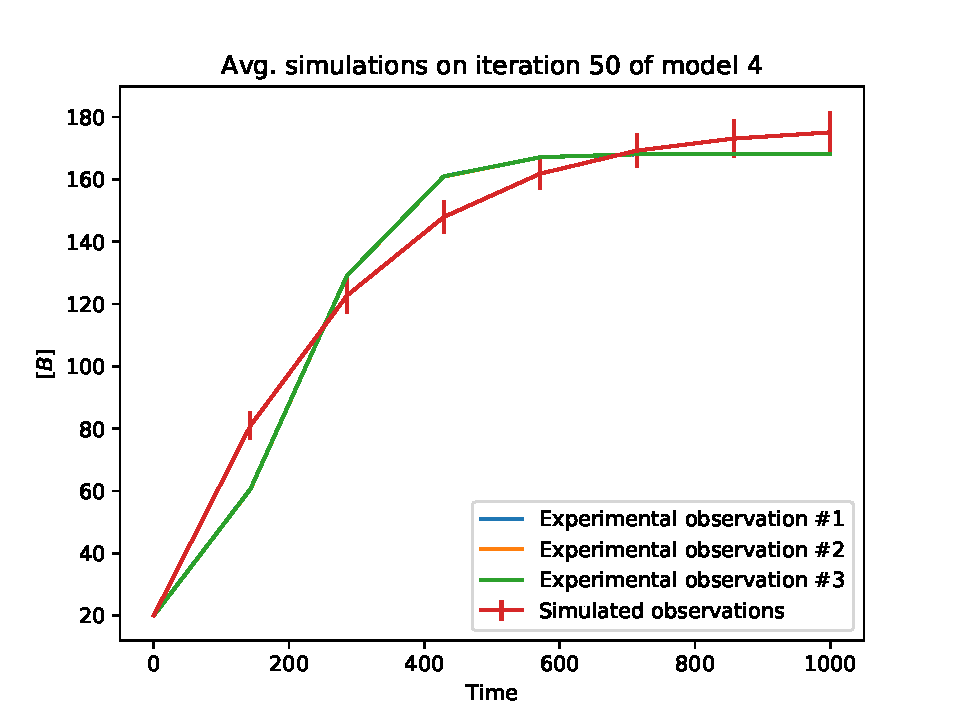
\includegraphics[clip=true,width=.6\linewidth]{experiments/results/smallest/simulations_model4_50.pdf}
    \label{fig:abc_sma_4it50}} 
    \end{tabular}
    \caption{Average simulation of iteration 50 for all candidate 
    models.}
    \label{fig:smallest_all_sim_it50}
\end{figure}

\begin{figure}[H]
    \centering
    \begin{tabular}{c c}
    \subfigure{
    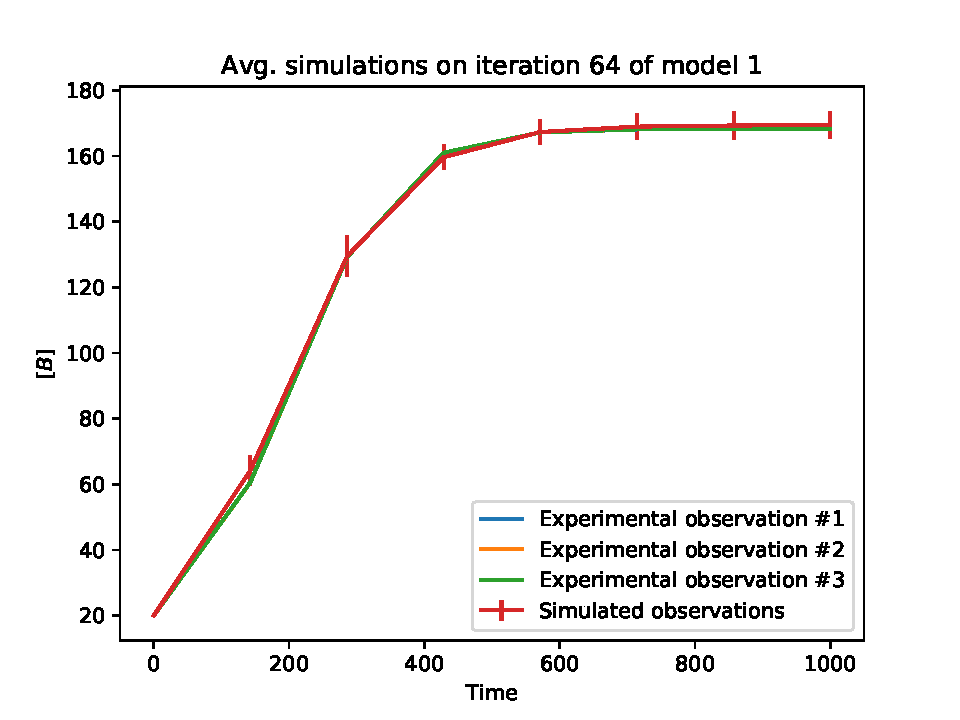
\includegraphics[clip=true,width=.45\linewidth]{experiments/results/smallest/simulations_model1_64.pdf}
    \label{fig:abc_sma_1it64}}
    &
    \subfigure{
    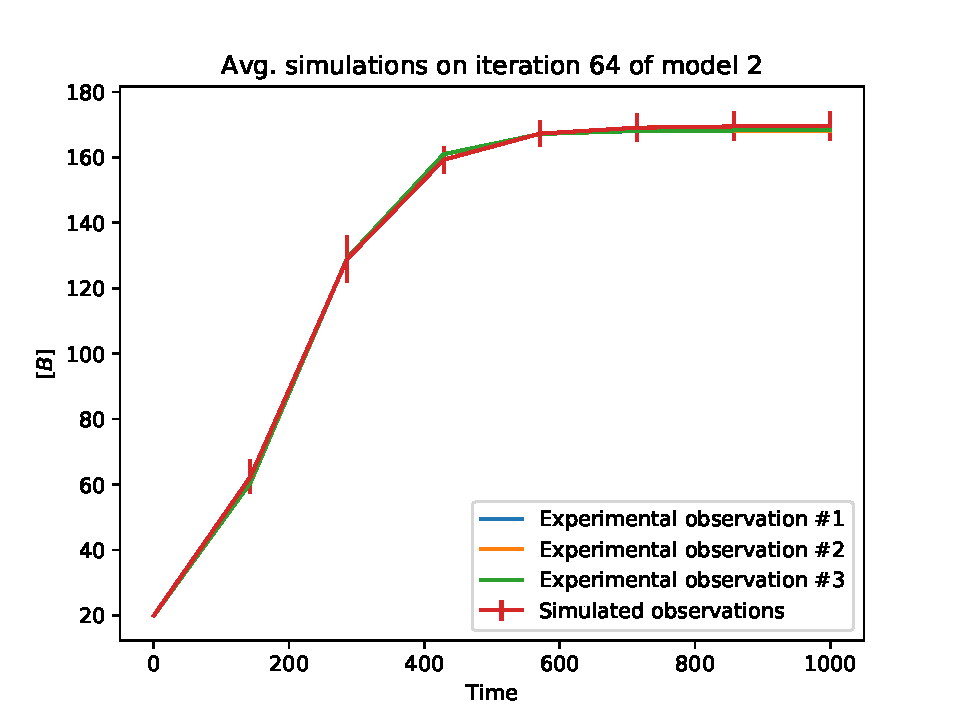
\includegraphics[clip=true,width=.45\linewidth]{experiments/results/smallest/simulations_model2_64.pdf}
    \label{fig:abc_sma_2it64}} 
    \end{tabular}
    \caption{Average simulation of iteration 20 for all candidate 
    models.}
    \label{fig:smallest_all_sim_it64}
\end{figure}

Since we achieved good results on the simulations of the model 1, we 
also plotted the estimation of the posterior distribution of the 
parameters given the data. Figure~\ref{fig:smallest_model1_posteriors}
shows the estimated posterior distribution for each parameter. We can 
note that the posterior distributions estimated have high density around
the true parameter values, i.e. parameter values used to create the
artificial experimental data.


\begin{figure}[p]
    \centering
    \begin{tabular}{c c}
    \subfigure{
    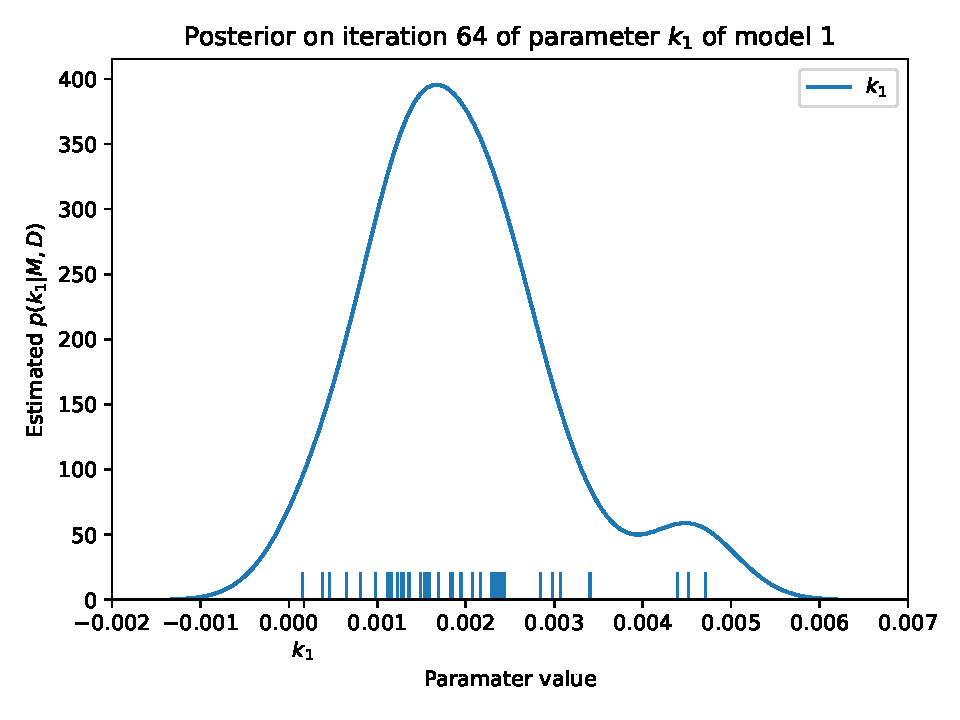
\includegraphics[clip=true,width=.45\linewidth]{experiments/results/smallest/model1_64_p0_k_1.pdf}
    }
    &
    \subfigure{
    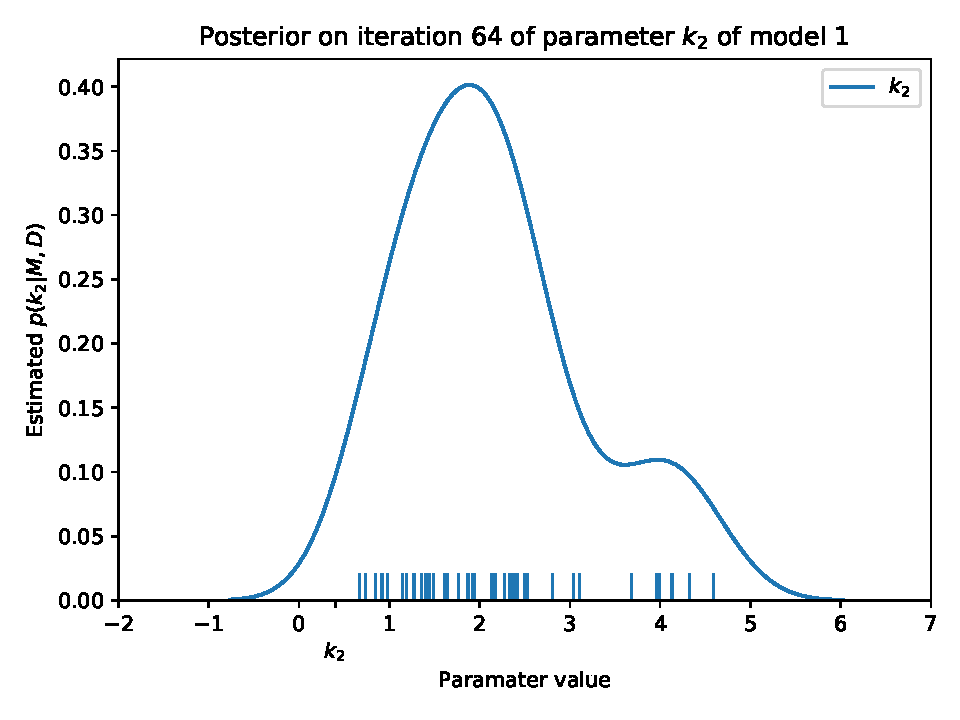
\includegraphics[clip=true,width=.45\linewidth]{experiments/results/smallest/model1_64_p1_k_2.pdf}
    }
    \\
    \subfigure{
    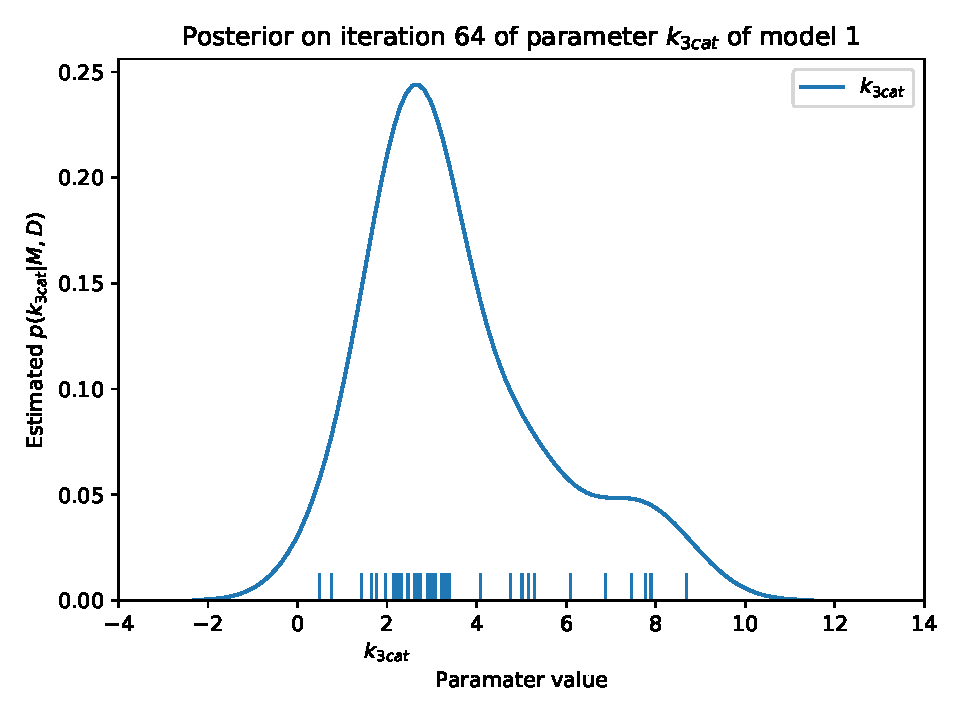
\includegraphics[clip=true,width=.45\linewidth]{experiments/results/smallest/model1_64_p2_k_3cat.pdf}
    }
    &
    \subfigure{
    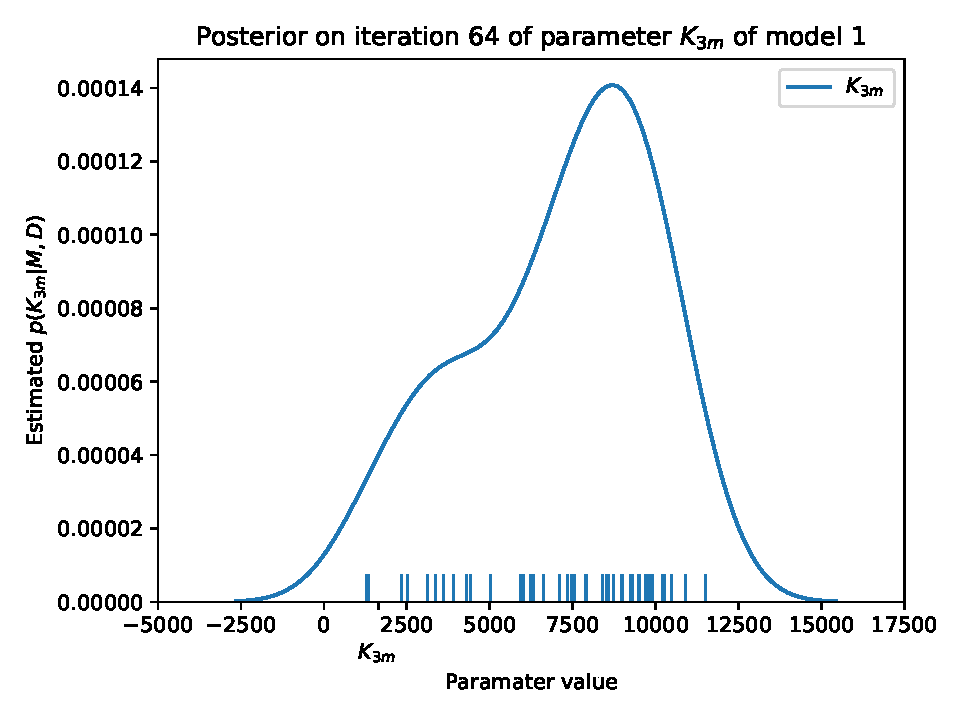
\includegraphics[clip=true,width=.45\linewidth]{experiments/results/smallest/model1_64_p3_K_3m.pdf}
    }
    \\
    \subfigure{
    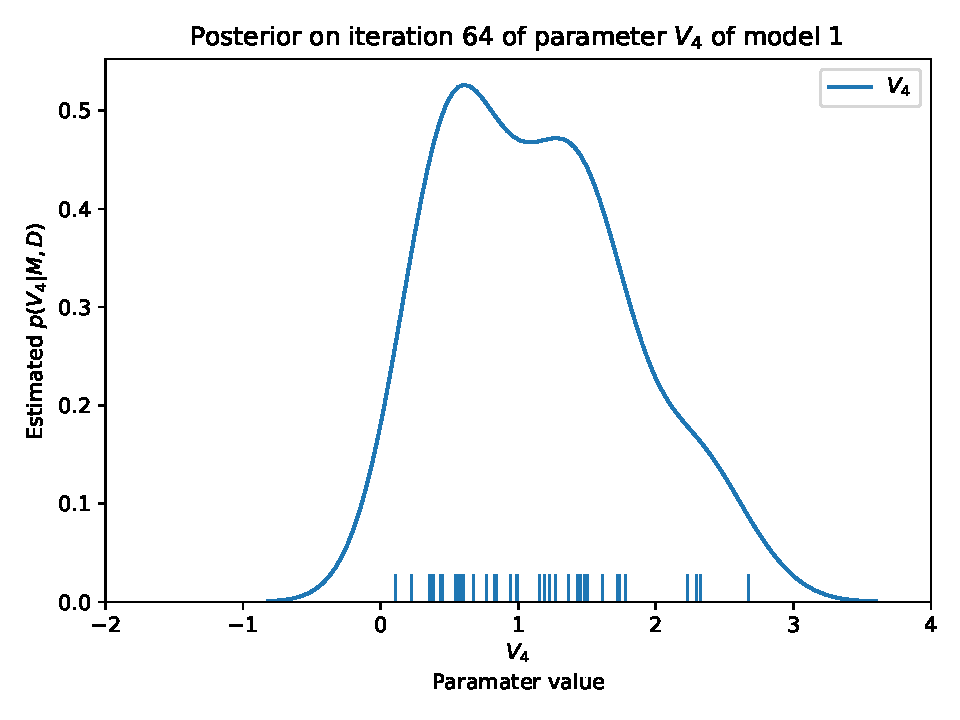
\includegraphics[clip=true,width=.45\linewidth]{experiments/results/smallest/model1_64_p4_V_4.pdf}
    }
    &
    \subfigure{
    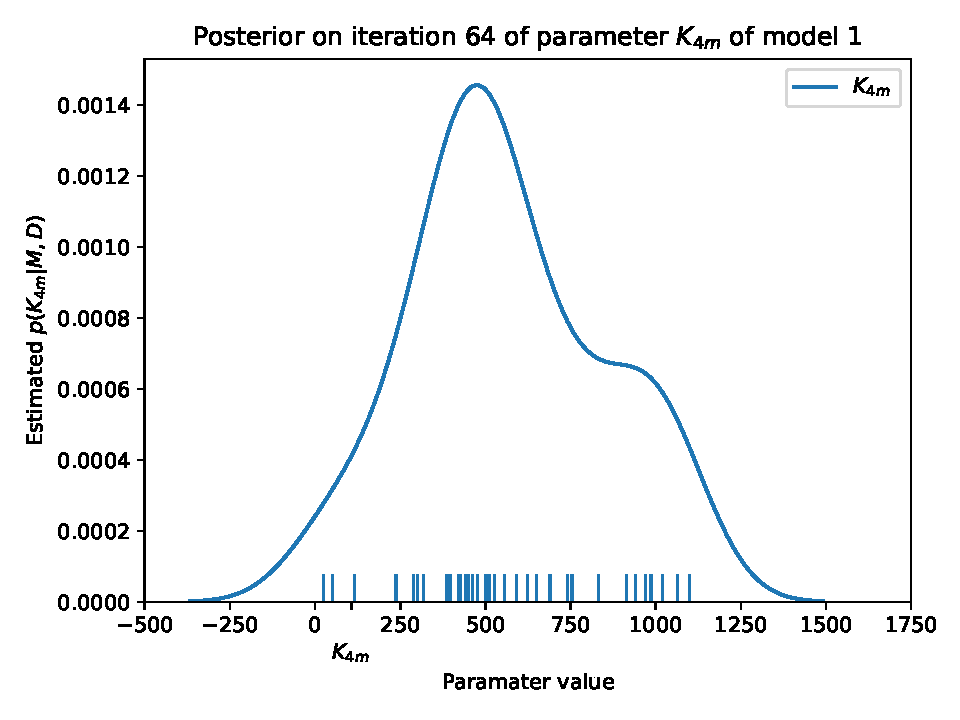
\includegraphics[clip=true,width=.45\linewidth]{experiments/results/smallest/model1_64_p5_K_4m.pdf}
    }
    \end{tabular}
    \caption{Estimates of the posterior distribution of model 1 
    parameters. These estimates were created using the kernel density 
    estimation method from the seaborn Python package. The parameter 
    name on the abscissa of the graph indicates the location of the 
    correct value of the parameter, i.e. the value used to create the 
    experimental data. The estimated posterior is not concentrated
    around the correct parameter values, which are $k_1 = 0.07$, 
    $k_2 = 0.6$, $k_3 = 0.05$, $k_4 = 0.3$, $V = 0.017$.}
    \label{fig:posterior_estimate_model1}
\end{figure}

